\chapter{水的三种状态}\label{ch:g6:water-states}

从二年级起，你就一直在追踪水的状态：
冰、水、水蒸气；融化的雪人和起雾的窗户。
今年，这场追踪变成了记账。冰融化时，
有没有物质丢失？水结冰时，为什么水管会爆裂？
手持天平和量筒，我们来核算水的三种状态。

\section{三种状态及其规范名称}

\begin{definition}[六种状态变化]\label{def:g6:water-states:changes}
水在三种状态之间有六条“通道”，每条都有
各自的科学名称：
  \begin{enumerate}
  \item 固态 $\to$ 液态：\emph{熔化}\index{熔化}；
        液态 $\to$ 固态：
        \emph{凝固}\index{凝固}（俗称结冰）；
  \item 液态 $\to$ 气态：\emph{汽化}\index{汽化}
        ——沸腾时剧烈进行，
        蒸发则安静而缓慢；气态 $\to$ 液态：
        \emph{液化}\index{液化}；
  \item 固态 $\to$ 气态（直接转化）：
        \emph{升华}\index{升华}，气态 $\to$ 固态
        ——这类通道较少见，却确实存在：窗上的霜花
        在冰冷的窗户上直接由看不见的水汽生长而成，
        完全跳过了液态。
\end{enumerate}
\end{definition}

\begin{omfigure}
\begin{tikzpicture}[scale=0.85]
  \node[draw, thick, omDef, font=\small, minimum width=1.9cm,
    minimum height=0.85cm] (ice) at (1.2,0) {冰};
  \node[draw, thick, omDef, font=\small, minimum width=1.9cm,
    minimum height=0.85cm] (wat) at (5.7,0) {水};
  \node[draw, thick, omDef, font=\small, minimum width=1.9cm,
    minimum height=0.85cm] (vap) at (10.2,0) {水汽};
  \draw[-Stealth, very thick, omThm] (2.25,0.28) -- (4.65,0.28);
  \node[above, font=\footnotesize, omThm] at (3.45,0.42) {熔化};
  \draw[-Stealth, very thick, omDef] (4.65,-0.28) -- (2.25,-0.28);
  \node[below, font=\footnotesize, omDef] at (3.45,-0.42)
    {凝固};
  \draw[-Stealth, very thick, omThm] (6.75,0.28) -- (9.15,0.28);
  \node[above, font=\footnotesize, omThm] at (7.95,0.42)
    {汽化};
  \draw[-Stealth, very thick, omDef] (9.15,-0.28) -- (6.75,-0.28);
  \node[below, font=\footnotesize, omDef] at (7.95,-0.42)
    {液化};
  \draw[-Stealth, very thick, omThm]
    (1.2,0.6) .. controls (3.0,2.1) and (8.4,2.1) .. (10.1,0.6);
  \node[above, font=\footnotesize, omThm] at (5.7,1.85)
    {升华};
\end{tikzpicture}

{\small 水的六条通道及其规范名称。暖意推动
红色通道；寒冷推动蓝色通道。}
\end{omfigure}

\begin{example}[身边的通道]\label{ex:g6:water-states:doors}
清晨草地上融化的霜；晾衣绳上的衣物正在蒸发；
冷镜子使你淋浴时的水汽凝结；冷冻室里
凝固着明天的冰块；霜花一夜之间长在
窗玻璃上。同一种物质，六条通道，都藏在
寻常的一天里——叫出它们的名字，你就真正掌握了它们。
\end{example}

\section{核算：物质会丢失吗？}

\begin{method}[称量状态变化]\label{met:g6:water-states:weigh}
用天平来检验这个问题：
\begin{enumerate}
  \item 把一些水倒进小塑料瓶，拧紧瓶盖，
        擦干外壁；
  \item 称重：读数为 \qty{368}{g}——记下来；
  \item 放进冷冻室过夜：凝固；
  \item 立即称量冷冻后的瓶子（擦去表面的霜）。
\end{enumerate}
天平的读数为 \qty{368}{g}，精确到克。把它放到窗台上
让它融化，再称一次：\qty{368}{g}。
状态变化了两次，物质的质量却毫无改变。
\end{method}

\begin{proposition}[状态变化不改变质量]\label{prop:g6:water-states:mass}
状态变化改变的是物质的外观，而不是
其量：变化前后的质量恰好相等。熔化、
凝固、在密闭锅中沸腾、凝结——每一条通道，
天平的读数都一样。（不过，若不盖紧瓶盖，
水汽会带着它的克数飘走：物质仍然存在，但你的
核算中已不再包含它。）
\end{proposition}

\begin{example}[水坑里的克数去哪儿了]\label{ex:g6:water-states:puddle}
一个 \qty{300}{g} 的水洼干了。消失了？称出来是零？不是：
\qty{300}{g} 的水现在以看不见的水汽飘在空中，每一克
都完好无损——有的将化作下周的雨落下。蒸发
骗得过眼睛，骗不过账本。你童年水坑实验里的
粉笔记号，其实就是一次核算；如今它有了数字。
\end{example}

\section{核算：体积保持不变吗？}

\begin{proposition}[水结冰时体积膨胀]\label{prop:g6:water-states:volume}
质量在各条通道中都不变，体积却不然。水是一种奇特的
物质：变成固体时，它会\emph{膨胀}。一升水
结成约 $1.1$ 升冰：质量相同，体积约多出十分之一。
大多数物质凝固时会收缩；水却会膨胀——
这一奇特性质会重塑地貌。
\end{proposition}

\begin{omfigure}
\begin{tikzpicture}[scale=0.85]
  \draw[thick] (1.2,0) -- (1.2,3.4) (3.0,0) -- (3.0,3.4)
    (1.2,0) -- (3.0,0);
  \fill[omDef, opacity=0.25] (1.2,0.05) rectangle (3.0,2.2);
  \draw[omDef, very thick] (1.2,2.2) -- (3.0,2.2);
  \node[below, font=\small] at (2.1,-0.3)
    {之前：水，\qty{368}{g}};
  \draw[thick] (7.0,0) -- (7.0,3.4) (8.8,0) -- (8.8,3.4)
    (7.0,0) -- (8.8,0);
  \fill[omDef, opacity=0.45] (7.0,0.05) rectangle (8.8,2.42);
  \draw[omDef, very thick] (7.0,2.42) -- (8.8,2.42);
  \draw[dashed, omExo] (7.0,2.2) -- (8.8,2.2);
  \node[below, font=\small] at (7.9,-0.3)
    {凝固后：冰，质量仍为 \qty{368}{g}};
  \draw[-Stealth, omThm, thick] (5.0,2.6) -- (6.8,2.45);
  \node[above, font=\small, omThm] at (5.0,2.65)
    {液面升高：体积增大，质量不变};
\end{tikzpicture}

{\small 冻结后的瓶子：天平示数不变，液面升高。
凝固保留了物质，却需要更多的空间。}
\end{omfigure}

\begin{example}[水管爆裂与山石开裂]\label{ex:g6:water-states:burst}
忘在冷冻室里的一瓶装满水的玻璃瓶裂开了：
膨胀的冰需要多出十分之一的空间，并把它占去，不论
瓶子是不是玻璃做的。冬天对水管也是如此：水在管中结冰，
会把管子胀裂，其力道不亚于一把铁锤——对山岳也一样：雨水
渗入岩缝，夜里结冰、膨胀，把
裂缝楔得更宽。年复一年，一次次冻结，
由\cref{prop:g6:water-states:volume}所说的那一点奇特膨胀，劈开巨石，
使山峰崩裂。
\end{example}

\begin{remark}[冰为什么会漂浮]\label{rem:g6:water-states:floats}
同样的这一奇特之处，也解答了你多年前洗澡时
问过的问题：同样是一升的物质，冰却要占去 $1.1$ 升的空间：
体积相同时，冰比水\emph{轻}，所以冰
会浮在自己的液体上。冰山漂浮在海面，池塘从上往下结冰
（让底下的鱼得以存活），柠檬水里的冰块也会浮起，
而不是下沉。很少有物质能浮在自身之上；冰封池塘里的生命
因为水有这一特性而感到庆幸。
\end{remark}

\section{水循环的账目核对}

\begin{example}[大循环，附词汇]\label{ex:g6:water-states:cycle}
童年里关于海洋、云和雨的故事，如今读来像一本
账簿。太阳的热量驱动海水\emph{汽化}
——数以吨计的水悄然升起。高空寒冷，水汽
\emph{凝结}成云滴；更冷时，水滴
凝固成雪。雪堆积成冰川，冰川\emph{熔化}
成河流；河流把每一克水都送回大海。绕行整个
循环，\cref{prop:g6:water-states:mass}始终成立：
地球既不增加也不减少一滴水——你杯中的水
早在恐龙时代之前，就已在这一循环中漂流。
\end{example}

\begin{omfigure}
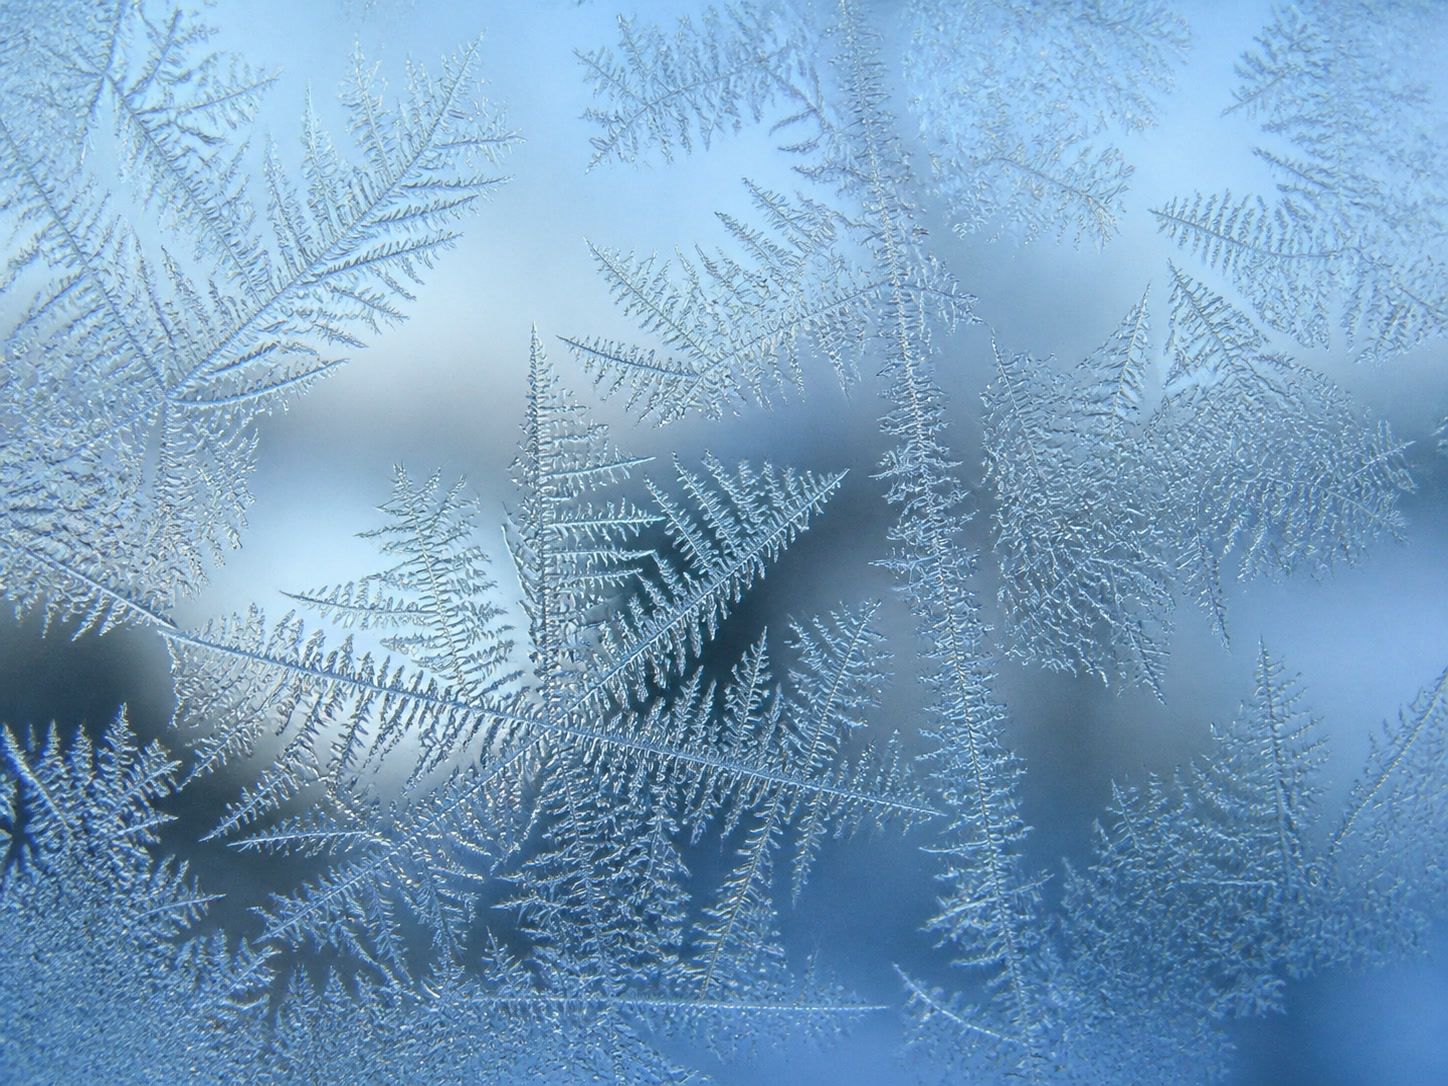
\includegraphics[width=0.5\linewidth]{images/book1/ai/g6-water-frost-window.jpg}

{\small 结冰的窗玻璃上长出的霜羽：空气中的水汽一夜之间直接在玻璃上结成了冰。}
\end{omfigure}

\section{练习}

\begin{exercise}[$\star$]\label{exo:g6:water-states:1}
说出\cref{def:g6:water-states:changes}中的六种状态变化，
各举一个日常所见的例子。
\end{exercise}

\begin{exercise}[$\star$]\label{exo:g6:water-states:2}
下面是哪种变化：清晨寒冷的草地上形成露水？\ 雪人
在晴朗的 \qty{-5}{\celsius} 天里缩小，却不见水洼出现？\ 冰块
让冷冻室里冒出“烟”一样的雾气？
\end{exercise}

\begin{exercise}[$\star$]\label{exo:g6:water-states:3}
一瓶密封的水的重量为 \qty{412}{g}。它完全凝固
了。一夜之后它的重量是多少？哪条命题可作解答？
\end{exercise}

\begin{exercise}[$\star$]\label{exo:g6:water-states:4}
在\cref{met:g6:water-states:weigh}中，瓶子为什么必须盖紧
——以及为什么每次称量前都要擦干？
\end{exercise}

\begin{exercise}[$\star$]\label{exo:g6:water-states:5}
一锅水敞口煮沸 10 分钟，它的质量减少了
\qty{200}{g}。质量被消灭了吗？这些克去了哪里？
\end{exercise}

\begin{exercise}[$\star$]\label{exo:g6:water-states:6}
一升水放入冷冻室，取出的冰大约有多大体积？
质量呢？同样的问题也请回答。
\end{exercise}

\begin{exercise}[$\star$]\label{exo:g6:water-states:7}
为什么严冬里水管会爆裂——园丁们为什么
要在秋天放掉户外水龙头里的水？
\end{exercise}

\begin{exercise}[$\star$]\label{exo:g6:water-states:8}
冰为什么会浮在水上？请把
\cref{prop:g6:water-states:volume}与漂浮规律联系起来——
在相同体积下，冰是更轻还是更重？
\end{exercise}

\begin{exercise}[$\star\star$]\label{exo:g6:water-states:9}
用账目的方式讲述水循环：跟踪 \qty{1}{kg} 海水
绕完整个循环，说出它经过的每种状态变化，并写出
它在每个阶段的质量。
\end{exercise}

\begin{exercise}[$\star\star$]\label{exo:g6:water-states:10}
一杯柠檬水满到杯口，冰块在里面上下浮动。
一位客人担心冰块融化时会溢出。请运用两条
核算（质量守恒，以及冰多出的空间被归还）来安抚
——或使其警觉——这位客人，并说明你的理由。
\end{exercise}

\begin{exercise}[$\star\star$]\label{exo:g6:water-states:11}
在干燥的房间里，一夜之间，结冰的窗玻璃上长出了霜羽，
睡前既没有下雨，窗玻璃也不湿。水经历的是哪种变化，
这些水从哪里来？为什么这种变化不叫
“凝固”？
\end{exercise}

\begin{exercise}[$\star\star\star$]\label{exo:g6:water-states:12}
池塘从上往下结冰。请解释整个过程：为什么
最冷的水的冰\emph{在表面}形成，并停留在那里，
浮冰之盖对下方的热量流动有什么影响（这是去年学过的一个
隔热思路），以及下面的鱼为何要感谢水的
奇特膨胀，才得以安然过冬。
\end{exercise}

\section{问题：环游世界的一千克水}

\begin{problem}[{周末问题 --- 一千克海水的环球之旅；
六扇门，三座山，一本不间断的
账本}]\label{pb:g6:water-states:1}
我们为 \qty{1}{kg} 海水贴上一张想象中的标签，并
跟踪它一年。

\medskip\noindent\textbf{第一部分 --- 上升。}
\begin{enumerate}
  \item 六月：太阳加热海面，我们的一千克水
        无形地升入空气中。说出它走的是哪一扇门。
  \item 这一千克（现已看不见的）水，其质量是多少？
        哪条命题
        保证了这一点？
  \item 在 \qty{3000}{m} 处，空气很冷：水变成一团
        小液滴组成的云。说出这扇门。
  \item 天气更冷时，小液滴变成雪花。说出这扇门
        的名称 --- 凝固 ---，并说明
        纯水云滴开始结冰的温度。
\end{enumerate}

\medskip\noindent\textbf{第二部分 --- 冰川的账目。}
我们的一千克水落到冰川上，并被压入冰川冰中。
\begin{enumerate}[resume]
  \item 作为水时，我们的一千克水占据 \qty{1}{L}。
        它作为冰时大约占据多大体积？
  \item 夏季时冰川的冰舌融化，我们的一千克水变为
        融水：它现在的质量是多少，其体积（还原为
        液态水后）是多少？
  \item 下山途中，我们的一千克水中有 \qty{250}{g}
        在阳光照耀的瀑布水潭里蒸发了。有多少
        被标记的水仍以液态留在溪流中？
  \item 蒸发掉的这四分之一是否已离开账目？说明它
        \qty{250}{g} 在何处，以及它们最可能
        接下来走哪扇门？
\end{enumerate}

\medskip\noindent\textbf{第三部分 --- 回家，
账目平衡。}
\begin{enumerate}[resume]
  \item 溪流中的 \qty{750}{g} 于十月抵达大海，
        被蒸发的 \qty{250}{g} 于八月在海岸上以雨的形式落下，
        于九月流入大海。算一算大海收回了
        我们这一千克水中的多少。
  \item 纵观整个旅程，我们的一千克水从未
        失重——但它两次\emph{看不见}。是在哪些
        阶段，以何种状态？
  \item 一位同学提出异议：“雪蓬松又轻，肯定
        这一千克水作为雪时更轻。”请用今年学过的
        一对正确术语，理清这个混淆。
  \item 将整个旅程按顺序写成一串门，只使用
        \cref{def:g6:water-states:changes}中的六个
        专有名称。
\end{enumerate}
\end{problem}
